\documentclass[preprint,review,12pt]{elsarticle}


%% Use the options 1p,twocolumn; 3p; 3p,twocolumn; 5p; or 5p,twocolumn
%% for a journal layout:
%% \documentclass[final,1p,times]{elsarticle}
%% \documentclass[final,1p,times,twocolumn]{elsarticle}
%% \documentclass[final,3p,times]{elsarticle}
%% \documentclass[final,3p,times,twocolumn]{elsarticle}
%% \documentclass[final,5p,times]{elsarticle}
%% \documentclass[final,5p,times,twocolumn]{elsarticle}

\usepackage{graphicx}% Include figure files
\usepackage{dcolumn}% Align table columns on decimal point
\usepackage{bm}% bold math
\usepackage{amssymb}
\usepackage{amsmath}


\newcommand{\lambdabar}{{\mkern0.75mu\mathchar '26\mkern -9.75mu\lambda}}

%% This list environment is used for the references in the
%% Program Summary
%%
\newcounter{bla}
\newenvironment{refnummer}{%
\list{[\arabic{bla}]}%
{\usecounter{bla}%
 \setlength{\itemindent}{0pt}%
 \setlength{\topsep}{0pt}%
 \setlength{\itemsep}{0pt}%
 \setlength{\labelsep}{2pt}%
 \setlength{\listparindent}{0pt}%
 \settowidth{\labelwidth}{[9]}%
 \setlength{\leftmargin}{\labelwidth}%
 \addtolength{\leftmargin}{\labelsep}%
 \setlength{\rightmargin}{0pt}}}
 {\endlist}

 \journal{Computer Physics Communications}

\begin{document}

\begin{frontmatter}

  \title{Capture cross section with quantum diffusion approach}

  \author[a,b]{V.V.Sargsyan}
  \author[a]{S.Yu.Grigoryev \corref{author1} }
  \author[a]{G.G.Adamian, \corref{author2}}
  \author[a]{N.V.Antonenko}

  \cortext[author1] {\\\textit{E-mail address:} grigorsu@gmail.com}
  \cortext[author2] {\\\textit{E-mail address:} adamian@theor.jinr.ru}

  \address[a]{Joint Institute for Nuclear Research, 141980 Dubna, Russia}
  \address[b]{Institut f\"ur Theoretische Physik der Justus--Liebig--Universit\" at, D--35392 Giessen, Germany}

  \date{\today}

  \begin{abstract}
  A C++ code for calculating the capture of a projectile by target nucleus is
  presented.  The model is based on the quantum diffusion approach developed for
  considering collisions of nuclei at energies below and just above the Coulomb barrier. 
  The code provides the capture cross sections and other characteristics as functions
  of $E_{\rm c.m.}$. The formalism of the model is briefly described.
  Also the code uses the Fortran subroutine to calculate the nucleus-nucleus potential.

  \end{abstract}


  \begin{keyword}
  sub-barrier fusion \sep dissipative dynamics \sep $S$-factor
  \PACS 25.70.Ji \sep 24.10.Eq \sep 03.65.-w

  \end{keyword}

\end{frontmatter}

{\bf\large PROGRAM SUMMARY}

\begin{small}
  \noindent
  {\em Title of program\/}: NeutronPairTransferCapture \\
  {\em Version\/}: 1.0 \\
  {\em Catalogue number\/}: \\
  {\em Program obtained from\/}: {\tt http://intel-robot.ru/external/www5/} \\
  {\em E-mail\/}: {\tt grigorsu@gmail.com, sargsyan@theor.jinr.ru} \\
  {\em License\/}: GNU Public License \\
  {\em Computers\/}: all \\
  {\em Operating system\/}: tested on Linux Ubuntu 14.04, 16.04,  Debian 8.0  \\
  {\em Compilator\/}: GNU Fortran (Debian 4.9.2-10) 4.9.2, g++ (Debian 4.9.2-10) 4.9.2, MinGW 4.9.2  \\
  {\em Program language\/}: {\tt C++, Fortran    } \\
  {\em Memory required to execute\/}: 
       depending on the complexity of the problem, 
       at least 64 MB RAM recommended   \\
  {\em Other programs called\/}: GSL-2.2.1 GNU Scientific Library in C++ is required.
       It is available from  {\tt https://www.gnu.org/software/gsl} .\\
  {\em External files needed\/}: none \\
  {\em Keywords\/}:  Neutron-pair transfer \\
  {\em Nature of the physical problem\/}: 
  ....\\
  {\em Method of solution\/}: 
  ....\\ 
  {\em Restrictions on complexity of the problem\/}: 
  Usually limited only by the available memory. \\
  {\em Typical running time\/}: several seconds up to 10 minutes, depending on HardWare.

% \begin{thebibliography}{0}
% \bibitem{1}Reference 1         % This list should only contain those items referenced in the                 
% \bibitem{2}Reference 2         % Program Summary section.   
% \bibitem{3}Reference 3         % Type references in text as [1], [2], etc.
%                                % This list is different from the bibliography at the end of 
%                                % the Long Write-Up.
% \end{thebibliography}

* Items marked with an asterisk are only required for new versions
of programs previously published in the CPC Program Library.\\
\end{small}


% main text ------------------------------------
\newpage

\section{Model}
\subsection{The capture cross}
\label{1}
  In our model the collision of nuclei is considered in terms of a single collective variable: the relative
  distance $R$ between the centers of colliding nuclei.
  Besides the dissipation of kinetic energy of the radial motion there is dissipation of angular momentum, i.e. the approach of the sticking limit \cite{VVV,Schreder}.
  Because the dissipation of angular momentum mainly occurs behind the Coulomb barrier, for simplicity, it can be disregarded to treat the passage of this barrier.
  The nuclear deformation effects are taken into consideration through the dependence
  of the nucleus-nucleus potential on the deformations and
  orientations of colliding nuclei. Thus, the total cross section of the
  capture of projectile by a target nucleus reads as the sum of partial capture cross sections
 

  \begin{eqnarray}
  &&\sigma_{\rm cap}(E_{\rm c.m.})=\sum_{L}^{}\sigma_{\rm cap}(E_{\rm c.m.},L)=\pi\lambdabar^2 \sum_{L}(2L+1)  \nonumber\\
   &\times&  \int_0^{\pi/2}d\theta_1\sin(\theta_1)\int_0^{\pi/2}d\theta_2\sin(\theta_2)P_{\rm cap}\left(E_{\rm c.m.},L,\theta_1,\theta_2\right)
  \label{1a_eq}
  \end{eqnarray}

  where $\lambdabar^2=\hbar^2/(2\mu E_{\rm c.m.})$ is the reduced de Broglie wavelength,
  $\mu=m_0 A_1 A_2/(A_1+A_2)$ is the reduced mass ($m_0$ is the nucleon mass), and the summation is in possible values of angular momentum $L$
  at given bombarding energy $E_{\rm c.m.}$.
  Knowing the potential of the interacting nuclei for each orientation at a given $L$, and the influence of intrinsic excitation of nuclei on the dynamics of
  relative distance $R$,  one can obtain the partial capture probability $P_{\rm cap}$, which is the probability of
  passing the potential barrier.
  In general case the capture probability $P_{\rm cap}$ is obtained by integrating the
  propagator $G$ from the initial state ($R_0, P_0$) at time $t = 0$ to
  the final state ($R,P$) at time $t$:
  \begin{eqnarray}
  P_{\rm cap}=\lim_{t\to\infty}\int_{-\infty}^{r_{\rm in}}dR\int_{-\infty}^{\infty}dP G(R,P,t|R_0,P_0,t=0).
  %=\lim_{t\to\infty}\frac{1}{2} {\rm erfc}\left[\frac{-r_{\rm in}+\overline{R(t)}}
  %{{\sqrt{\Sigma_{RR}(t)}}}\right].
  \label{PcapG}
  \end{eqnarray}
  Here, $r_{\rm in}$ is the internal turning point of the nucleus-nucleus potential
  $V(R,Z_i, A_i,\theta_i,L)$ for $E_{\rm c.m.}$ smaller than the height $V_b=V(R_b,Z_i, A_i,\theta_i,L)$
  of the Coulomb barrier. To obtain analytical expressions for the capture cross-section, we
  use the following procedure. For each angular momentum $L$ and given orientation angles $\theta_i$, the realistic nucleus-nucleus potential is calculated and the classical action is found for this potential.
  Then the value of $P_{\rm cap}\left(E_{\rm c.m.},L,\theta_1,\theta_2\right)$ is analytically
  calculated for the inverted oscillator potential which has the same barrier height $V_b$ and
  classical action. So, the frequency $\Omega$ of this oscillator is defined from the condition of equality of the
  classical actions and depends on $E_{\rm c.m.}$, $L$, and $\theta_i$.
  If the initial energy of colliding nuclei is above the potential barrier at $R=R_b$, then we set
  $\Omega=\sqrt{\left.-\dfrac{1}{\mu}\dfrac{\partial^2 V(R)}{\partial R^2}\right|_{R_b}}$.

  As shown in Ref.~\cite{DMDadonov}, in the case of inverted oscillator the propagator $G$ has the following form:
  \begin{eqnarray}
  G=\pi^{-1}|\det {\bf \Sigma}^{-1}|^{1/2} \exp(-{\bf q}^{T}{\bf \Sigma}^{-1}{\bm q})
  \label{prop}
  \end{eqnarray}
  where
  $q_R(t)=R-\overline{R(t)}$, $q_P(t)=P-\overline{P(t)}$, $\overline{R(t=0)}=R_0$,
  $\overline{P(t=0)}=P_0$, $\Sigma_{ij}(t)=2\overline{q_i(t)q_j(t)}$, $\Sigma_{ij}(t=0)=0$,
  $i,j=R,P$.
  Using Eqs.~(\ref{PcapG}) and (\ref{prop}), we find a simple expression for the capture cross-section:
  \begin{eqnarray}
  P_{\rm cap}=\lim_{t\to\infty}\frac{1}{2} {\rm erfc}\left[\frac{-r_{\rm in}+\overline{R(t)}} {{\sqrt{\Sigma_{RR}(t)}}}\right].
  \label{propPcap}
  \end{eqnarray}
  So, the main ingredients of our calculation are the nucleus-nucleus potential and
  time dependencies of $\overline{R(t)}$ and $\Sigma_{RR}(t)$.

\subsection{The nucleus-nucleus potential}

  The potential describing the interaction of two nuclei can
  be written in the form \cite{poten}
  \begin{eqnarray}
  V(R,Z_i, A_i,\theta_i,L)=V_{\rm C}(R,Z_i, A_i,\theta_i)+V_{\rm N}(R,Z_i, A_i,\theta_i)+\frac{\hbar^2 L(L+1)}{2\mu R^2},
  \label{pot}
  \end{eqnarray}
  where $V_{\rm N}$, $V_{\rm C}$, and the last summand stand for the nuclear,
  the Coulomb, and the centrifugal potentials, respectively.
  The nuclei are proposed to be spherical or deformed. The
  potential depends on the distance $R$ between the center of
  mass of two interacting nuclei, mass $A_i$ and charge $Z_i$ of
  nuclei ($i = 1, 2$), the orientation angles $\theta_i$ of the deformed
  (with the quadrupole deformation parameters $\beta_i$) nuclei
  and the angular momentum $L$.

  For the nuclear part of $V$, we use the double-folding formalism
  \begin{eqnarray}
  V_{\rm N}=\int\rho_1(\bold {r_1})\rho_2(\bold{R}-\bold{r_2})F(\bold{r_1}-\bold{r_2})d\bold{r_1}d\bold{r_2},
  \label{vn}
  \end{eqnarray}
  where
  $F(\bold {r_1}-\bold{r_2})=C_0[F_{\rm in}\frac{\rho_0(\bold{r_1})}{\rho_{00}}+F_{\rm
  ex}(1-\frac{\rho_0(\bold{r_1})}{\rho_{00}})]\delta(\bold{r_1}-\bold{r_2})$
  is the density-depending effective nucleon-nucleon interaction and $\rho_0(\bold{r})=\rho_1(\bold{r})+\rho_2(\bold{R}-\bold{r})$,
  $F_{\rm in,ex}=f_{\rm in,ex}+f_{\rm in,ex}^{'}\frac{(N_1-Z_1)(N_2-Z_2)}{(N_1+Z_1)(N_2+Z_2)}$,
  $\rho_1(\bold{r_1})$, $N_1$, $Z_1$ and $\rho_2(\bold{r_2})$, $N_2$, $Z_2$ are the nucleon
  densities, neutron numbers, charge numbers of, respectively, the projectile and the target
  nucleus.
  Note, that the parameters of effective nucleon-nucleon interaction are fixed and set:
  $C_0=$ 300 MeV fm$^3$, $f_{\rm in}=$ 0.09, $f_{\rm ex}=$ -2.59, $f_{\rm in}^{'}=$ 0.42, $f_{\rm ex}^{'}=$ 0.54 and $\rho_{00}=$0.17 fm$^{-3}$.
  The nucleus-nucleus potential \cite{poten} used here naturally contains the repulsive part because of the
  density-dependent nucleon-nucleon forces in Eq.~(\ref{vn}). Note, that as the centrifugal part of the potential grows, the pocket depth becomes smaller and the position of the potential pocket minimum moves towards the barrier
  of the hight $V_b=V(R_b)$ at $R=R_b$.
  The value of $R_b$ is approximately equal to $R_1+R_2+2$ fm where $R_1$ and $R_2$ are the radii of colliding nuclei,
  $R_i=r_0A_i^{1/3}$. The program provides us the values of $V_b$ and $R_b$ for spherical
  nuclei. Because there are some uncertainties
  in the calculation of the potential, the program allows us also to enter the user value of $V_b$ for spherical
  nuclei. In this case the calculated nucleus-nucleus potential is correspondingly shifted.

  The densities of the nuclei are taken in the two-parameter symmetrized Woods-Saxon form.
  The nuclear radius parameter $r_0$ and the diffuseness parameters $a_i$ can depend on the charge and mass
  numbers of the nuclei \cite{poten}.

  The Coulomb interaction of two deformed nuclei with the quadrupole deformation parameters $\beta_i$
  is as follows
  \begin{eqnarray}
  &&V_{\rm C}(R,Z_i, A_i,\theta_i)=\frac{Z_1 Z_2 e^2}{R}  \nonumber\\
  &+& 
  \left(\frac{9}{20 \pi}\right)^{1/2}\frac{Z_1 Z_2 e^2}{R^3}\sum_{i=1,2}R_i^2\beta_i\left[1+\frac{2}{7} \left(\frac{5}{\pi}\right)^{1/2} \beta_i\right] P_2(\cos\theta_i)
  \end{eqnarray}
  where $P_2(\cos\theta_i)$ is the Legendre polynomial.

  In the calculations of nucleus-nucleus potential the parameters of effective nucleon-nucleon interaction are fixed for all nuclei. We set the nuclear radius parameter $r_0=1.15$ fm and the diffuseness parameter $a=0.48$ fm for the He, $a=0.5$ fm for the Li, $a=0.53$ fm for $4\leq Z \leq 9$,
  $a=0.55$ fm for $10\leq Z \leq 88$ and $a=0.56$ fm for $Z \geq 89$.

  %As follows from our calculations, the dissipation of orbital angular momentum causes
  %the decrease of the value of potential $V(R)$. However, the value of $\partial V(R)/\partial R$ is only slightly changed in the reactions considered.
  %Thus, considering the decay or reflection from the region behind the barrier, one can use the potential at fixed angular momentum for bombarding energies of interest.

\subsection{Quantum non-Markovian dynamics}

  The Hamiltonian $H$ of two colliding nuclei explicitly depends on $R$, the canonically
  conjugate collective momentum $P$, and the internal
  degrees of freedom \cite{Leggett,Jolos}. If the coupling between the collective subsystem and the
  thermostat is realized in terms of the collective coordinate $R$ and the internal coordinates $q_{\nu}$, then the total
  Hamiltonian of the system is written as
  \begin{eqnarray}
  H&=&H_c+H_b+H_{cb},\nonumber\\
  H_c&=&\frac{1}{2\mu}P^2-\frac{\mu\omega^2}{2}R^2,\nonumber\\
  H_b&=&\sum_{\nu}^{}\hbar\omega_\nu b_\nu^+b_\nu,\nonumber\\
  H_{cb}&=&\frac{\kappa}{\hbar}\lambda^{1/2}R\sum_{\nu}^{}\Gamma_\nu(b_\nu^+ + b_\nu)
  +\frac{\kappa^2}{\hbar^2}\lambda R^2\sum_{\nu}^{}\frac{|\Gamma_\nu|^2}{\hbar\omega_\nu}.
  \label{1_eq}
  \end{eqnarray}
  Here, $b_\nu^+$ and $b_\nu$ are the phonon creation and annihilation operators describing the internal
  excitations at energy $\hbar \omega_\nu$. The operators $H_{c}$ and $H_{b}$
  are the Hamiltonians of the collective and internal subsystems, respectively. The first term in $H_{cb}$ describes
  the coupling between the collective motion and the internal excitations and is the source of the dissipation
  term in the equations for the operators of collective variables. For example, in the description of nuclear
  interaction at low energies, this term corresponds to the effect of the mean field of each nucleus on the
  one-particle motion in other nucleus. In Eq.~(\ref{1_eq}), $\Gamma_\nu$ is the coupling constant between the collective
  subsystem and the internal coordinates, and $\lambda$ is a parameter determining an average force of
  coupling to the thermostat, $\kappa=(2\mu\omega\lambda/\hbar)^{1/2}$. The additional term in $H_{cb}$ compensates for the potential
  renormalization appearing because the collective and internal subsystems are coupled \cite{Leggett}. Our aim is to
  derive and analytically solve the Langevin equations for the collective operators $R$ and $P$. The quadratic
  Hamiltonian admits an exact solution of the equations of motion for the collective coordinates.

  Using Hamiltonian (\ref{1_eq}), we obtain the system of integro-differential stochastic equations
  (the system of generalized nonlinear Langevin equations) \cite{VAZ}
  \begin{eqnarray}
  \dot R(t)&=&\frac{P(t)}{\mu},\nonumber\\
  \dot P(t)&=&-\mu \omega^2 R(t) - \kappa^2\int\limits_{0}^{t}d\tau K(t-\tau)\dot R(\tau) + \kappa F(t).
  \label{4_eq}
  \end{eqnarray}
  The integral term in these equations
  means that the considered system is non-Markovian and has some “memory” over the trajectory
  preceding the instant $t$. As seen from the equation for $P(t)$, the coupling term of the Hamiltonian
  results in the random momentum-related force,
  \begin{eqnarray}
  F(t)&=&F_p(t)/\kappa=-\frac{\lambda^{1/2}}{\hbar}\sum_{\nu}^{}
  \Gamma_\nu[f_\nu^{+}(t)+f_\nu(t)]=\sum_{\nu}^{}F^{\nu}(t),\nonumber\\
  f_\nu^+(t)&=&[b_\nu^+(0)+\frac{1}{\hbar^2\omega_\nu}\kappa\lambda^{1/2}\Gamma_\nu]e^{i\omega_\nu t},
  \label{rand}
  \end{eqnarray}
  and a dissipation kernel,
  \begin{eqnarray}
  K(t-\tau)=\frac{2\lambda}{\hbar^2}\sum_{\nu}^{}
  \frac{\Gamma_\nu^2}{\hbar\omega_\nu}\cos(\omega_\nu[t-\tau]).
  \label{kern}
  \end{eqnarray}
  As seen from Eqs.~(\ref{rand}) and (\ref{kern}), the random force and the dissipation kernel are independent
  of the dynamical coordinates and momenta. The temperature and fluctuations are related to
  the distribution of the initial coordinates and momenta in the internal subsystem (at $t = 0$).
  The random force operators $F^{\nu}$ are identified with the fluctuations
  because the initial conditions for the thermostat operators are ambiguous.
  These fluctuations have zero mean values and nonzero variances \cite{Katia}.

  To solve Eqs.~(\ref{4_eq}) analytically, we use the Laplace transform method. After finding expressions for the
  images, we obtain explicit expressions for the originals,
  \begin{eqnarray}
  R(t)=A_t R(0)+B_t P(0)+\kappa\int\limits_{0}^{t}d\tau B_\tau F(t-\tau),\nonumber\\
  P(t)=M_t R(0)+N_t P(0)+\kappa\int\limits_{0}^{t}d\tau N_\tau F(t-\tau),
  \label{7_eq}
  \end{eqnarray}
  where
  \begin{eqnarray}
  B_t&=&\frac{1}{\mu} {\cal L}^{-1}\left[\frac{1}{s^2+2\hbar\omega sK(s)+\tilde\delta/\mu}\right],\nonumber\\
  A_t&=&{\cal L}^{-1} \left[\frac{s+2\hbar\omega K(s)}{s^2+2\hbar\omega sK(s)+\tilde\delta/\mu}\right]=
  \mu\dot B_t + \kappa^2\int\limits_{0}^{t}d\tau B_\tau K(t-\tau),\nonumber\\
  M_t&=&-\mu{\tilde \delta} B_t,\nonumber\\
  N_t&=&\mu\dot B_t.
  \label{ABfun}
  \end{eqnarray}
  Here, ${\cal L}^{-1}$ denotes the inverse Laplace transform, and $K(s)$ is the image of the dissipation kernel $K(t)$.
  The symbols $t$ and $\tau$ indicate the temporal dependence and $\tilde{\delta}=-\mu\omega^2$.

  As follows from Eq.~(\ref{propPcap}), to obtain the capture cross-section one need to know the first and second moments for the collective coordinate $R(t)$:
  $\overline{R(t)}$ and $\Sigma_{RR}(t)$.
  From Eq.~(\ref{7_eq}) we have for the first moments
  \begin{eqnarray}
  \overline{R(t)}=A_t\overline{R(0)} + B_t \overline{P(0)}, \nonumber\\
  \overline{P(t)}=M_t \overline{R(0)} + N_t \overline{P(0)},
  \label{8_eq}
  \end{eqnarray}
  and for the second moment
  \begin{eqnarray}
  \frac{1}{2}\Sigma_{RR}(t)&=&\sigma_{RR}=\overline{R(t)^2}-\overline{R(t)}\ ^2\nonumber\\
  =A_t^2\sigma_{RR}(0)&+&A_t B_t\sigma_{RP}(0)+B_t^2\sigma_{PP}(0)+J_{RR}(t)
  %\label{8_eq}
  \end{eqnarray}
  where
  \begin{eqnarray}
  J_{RR}(t)&=&\frac{2\omega\mu\lambda}{\hbar}
  \sum_{\nu}^{}|\Gamma_\nu|^2\coth\left[\frac{\hbar\omega_\nu}{2T}\right]  \nonumber\\
&\times& \int\limits_{0}^{t}
  d\tau^{'}B_{\tau^{'}}  \int\limits_{0}^{t} d\tau^{''}B_{\tau^{''}}
  \cos[\omega_\nu (\tau^{'}-\tau^{''})].
  \label{Jrr}
  \end{eqnarray}
  To set the initial energy of the colliding nuclei, we take $\sigma_{RR}(0)=\sigma_{RP}(0)=\sigma_{PP}(0)=0$.
  To define the initial values of $\overline{R(0)}$ and $\overline{P(0)}$, we consider two regime of interactions.
  At large $R$, where the nuclei are well separated, 
  the friction does not play a significant role. When the nuclei approach each other,
  the dynamics of the colliding nuclei strongly depends on friction and diffusion. 
  So, the dependence of friction on $R$ is taken in a simple way.
  The interaction parameter $R=R_{\rm int}=1.1$ fm is introduced. If the initial energy of colliding nuclei is less than
  $E_{\rm c.m.}<V(R_b+R_{\rm int})$, we set $\overline{P(0)}=0$ and find $\overline{R(0)}$ from the equality 
  $$-\dfrac{\mu \Omega^2}{2}\overline{R(0)}^2=E_{\rm c.m.}-V_b.$$
  In this case the friction plays a negligible role in the transition through the
  barrier.
  If $E_{\rm c.m.}>V(R_b+R_{\rm int})$, we set $\overline{R(0)}=R_{\rm int}$ and find $\overline{P(0)}$ 
  from the condition
  $$\dfrac{\overline{P(0)}^2}{2 \mu}-\dfrac{\mu \Omega^2}{2}R_{\rm int}^2=E_{\rm c.m.}-V_b.$$

  To obtain analytical expressions, in the expressions above the sums $\sum_{\nu}^{}...$ are replaced by the
  integral $\int\limits_{0}^{\infty} dw g(w)...$ over the frequency with the density $g(w)$ of states  for
  the thermostat (see \cite{Katia,VAZ}). So,
  $$\frac{g(w)|\Gamma (w)|^2}{\hbar^2w}= \frac{\gamma^2}{\pi (\gamma^2+w^2)},$$
  and
  $$K(t)=\frac{\lambda\gamma}{\hbar}e^{-\gamma|t|}$$
  from Eq.~(\ref{kern}). This choice of $g(w)$ is justified because it results in the Markovian limit at $\gamma\rightarrow\infty$.
  Substituting the image $$K(s)=\frac{\lambda\gamma}{\hbar (s+\gamma)}$$ of the dissipation kernel in (\ref{ABfun}) and (\ref{Jrr}), we obtain
  \begin{eqnarray}
  B_t=\sum_{i=1}^{3}B_t^i=\frac{1}{\mu}\sum_{i=1}^{3}\beta_i(s_i+\gamma)e^{s_it},\nonumber\\
  A_t=\sum_{i=1}^{3}\beta_i[s_i(s_i+\gamma)+2\omega\lambda\gamma]e^{s_it},
  \label{ABroot}
  \end{eqnarray}
   \begin{eqnarray}
  J_{RR}(t)&=&\frac{2\omega\lambda}{\pi\mu} \int\limits_{0}^{\infty} dw\frac{\gamma^2  w}{\gamma^2+w^2}\coth(\hbar w/(2T))\times \nonumber\\
&\times&  \sum_{i,j}\beta_i\beta_j(s_i+\gamma)(s_j+\gamma)\psi(s_i,s_j,w,t),
  \label{sigma}
  \end{eqnarray}
  where $s_i$, $i=1,2,3$, are the roots of the equation
  \begin{eqnarray}
  (s+\gamma)(s^2-\omega^2)+2\omega\lambda\gamma s=0,
  \label{roots2}
  \end{eqnarray}
  where  $\beta_1=1/[(s_1-s_2)(s_1-s_3)]$,  $\beta_2=1/[(s_2-s_1)(s_2-s_3)]$, $\beta_3=1/[(s_3-s_1)(s_3-s_2)]$,
  and
  \begin{eqnarray}
  \psi(s_i,s_j,w,t)=\int\limits_{0}^{t} d\tau^{'}e^{s_i \tau^{'}} \int\limits_{0}^{t} d\tau^{''}e^{s_j \tau^{''}}
  \cos[w (\tau^{'}-\tau^{''})],
  \label{expint}
  \end{eqnarray}
  can be analytically calculated.
  Note, that Eqs.~(\ref{8_eq}) and (\ref{sigma}) with Eq.~(\ref{ABroot}) completely determine the dynamics of collective subsystem. They are used to find $\overline{R(t)}$ and $\Sigma_{RR}(t)$.

  Because the relaxation time for the internal subsystem is much shorter than
  that for collective motion, the condition $\gamma\gg \Omega$ should be fulfilled.
  Note, that the non-Markovian effects appear in the calculations through the internal-excitation width $\gamma$.
  This parameter characterizes the density of nuclear states.
  We set $\hbar\gamma=12$ MeV for the nuclei $4\leq Z \leq 88$ and  $\hbar\gamma=24$ MeV for $Z\geq89$.

\subsection{Asymptotic expressions }

  In the case of inverted oscillator, Eq.~(\ref{roots2}) has three real roots, one positive ($s_1>0$) and two negative ($s_2,s_3<0$).
  This means that in practical calculations of the first (\ref{8_eq}) and second (\ref{sigma}) moments one can
  consider only the leading term,
  proportional to $\sim e^{s_i t}$.
  In this case the integral Eq.~(\ref{expint}) leads to $\dfrac{e^{2 s_1 t}}{s_1^2+w^2}$ and for large $t$ we obtain
  \begin{eqnarray}
  \Sigma_{RR}(t)&=& e^{2 s_1 t}\frac{4 \omega \lambda\gamma^2}{\pi \mu}\beta_1^2(s_1+\gamma) \nonumber\\
  &\times& \left[\frac{\pi T}{s_1\gamma}+\frac{1}{s_1-\gamma}
  \left[\psi^{0}\left(1+\frac{s_1}{2\pi T}\right)-\psi^{0}\left(1+\frac{\gamma}{2\pi T}\right)\right]\right],
  \label{sigmaAs}
  \end{eqnarray}

  where
  \begin{eqnarray}
  \psi^{0}(z)=\frac{\Gamma^{'}(z)}{\Gamma(z)}
  \end{eqnarray}
  is the di-gamma function.

  The total Hamiltonian (\ref{1_eq}) contains the coupling parameter $\lambda$ and frequency $\omega$. These values
  are defined through the correspondence to the realistic transport coefficients.
  The transport coefficients are found from Eq.~(\ref{7_eq}) by differentiating in time and expressing $\overline{R(0)}$ and $\overline{P(0)}$  in terms of $\overline{R(t)}$ and $\overline{P(t)}$:
  \begin{eqnarray}
  \frac{d}{dt}\ \overline{R(t)}&=&\frac{1}{\mu}\ \overline{P(t)},\nonumber\\
  \frac{d}{dt}\ \overline{P(t)}&=&-\xi (t)\ \overline{R(t)}-\lambda_P(t)\ \overline{P(t)}.
  \label{14_eq}
  \end{eqnarray}
  From the structure of these equations one can identify the time dependent friction coefficient
  \begin{eqnarray}
  \lambda_P(t)=\frac{A_t{\dot N}_t - B_t{\dot M}_t }
  {B_tM_t - A_tN_t},
  \label{15b_eq}
  \end{eqnarray}
  and the renormalized stiffness coefficient
  \begin{eqnarray}
  \xi (t) = \frac{{\dot M}_t N_t - {\dot N}_tM_t}
  {B_tM_t - A_tN_t}.
  \label{15d_eq}
  \end{eqnarray}
  For the asymptotic values of the friction and stiffness
  we obtain the expressions
  \begin{eqnarray}
  \nonumber
  \lambda_P(\infty)&=&-(s_2+s_1),\\
  \xi (\infty)&=&\tilde\delta\frac{(s_1+\gamma)(s_2+\gamma)}{(s_1+\gamma)(s_2+\gamma)-
  2\lambda\gamma\omega}
  \label{as_trans}
  \end{eqnarray}
  where $s_2>s_3$. The parameters $\omega$ and $\lambda$ in Eq.~(\ref{1_eq}) are chosen in such a way that the asymptotic values of friction and stiffness (\ref{as_trans}) take the values $\lambda_P(\infty)=2$ MeV and $\xi (\infty)=-\mu \Omega^2$. As known \cite{PRC1,PRC2}, the realistic friction coefficients are in the range of $1-2$ MeV.
  These values are close to those obtained within the mean-field approaches \cite{Wash,Ayik1}.


\section{Role of neutron transfer in capture processes}
  The importance of the neutron transfer, if the corresponding $Q_{2n}$-value is positive, in nuclear capture (fusion) originates from the fact
  that neutrons are insensitive to the Coulomb barrier and their transfer can start at large separations, before the
  projectile is captured by the target nucleus \cite{Stelson,NashiTrs,Broglia}.
  If the two-neutron transfer occurs before crossing the Coulomb barrier, it can lead to the population
  of the first $2^{+}$ state in the recipient nucleus \cite{Szilner}. So, the motion
  to the $N/Z$ equilibrium starts in the system before the capture.
  The average change of mass asymmetry is connected to the two-neutron transfer. Because after two-neutron transfer the
  mass numbers, the deformation parameters of the interacting nuclei, and, correspondingly, the height and shape of the
  Coulomb barrier are changed, one can expect an enhancement or suppression of the capture.
  After two-neutron transfer the residues of donor nuclei is assumed to remain in the
  ground state with the corresponding quadrupole deformation.
  For sub-barrier energies, the results of calculations are very
  sensitive to the quadrupole deformation parameters $\beta_2$ of the interacting nuclei. The quadrupole deformation parameters  $\beta_2$
  are taken from Ref.~\cite{Raman} for deformed even-even nuclei. In Ref.~\cite{Raman}, the quadrupole deformation parameters  $\beta_2$
  are given for the first excited $2^{+}$ states of nuclei. For the nuclei deformed
  in the ground state, the $\beta_2$  in $2^{+}$ state is similar to that in the ground state and we
  use $\beta_2$ from Ref.~\cite{Raman} in the calculations.
  For double magic nuclei and neighboring nuclei, in the ground state we take $\beta_2=0$. The program takes
  $\beta_i$ from the data file incorporated and allows 
  us also to input the user values of $\beta_i$.

\section{The program}
\label{sec:design}

  The program is located in the folder \textit{QDA}. It has the following structure: 
  
  \begin{itemize}
    \setlength\itemsep{0em}
    \item[QDA/run/]    - The program consist of three scripts from this folder: settings.exe, fort.exe and pcapt.exe. Files \textit{settings.exe} and \textit{pcapt.exe} are compiled from files \textit{QDA/source/settings.cc} and \textit{QDA/source/pcapt.cc}. The file fort.exe is compiled from files \textit{P1.FOR P2.FOR P3.FOR P4.FOR} from the folder \textit{QDA/source/} There is a friendly user interface on webpage Ref.~\cite{WebInterface}. 
    \item[conf/]   - contains config file isotopes.table.txt. This file is used to define nuclear properties (mass, quadrupole deformation parameters $\beta$, .. ) by charge $Z$ and weight $A$. Here is its part:
\begin{verbatim}
 Z    A     m(KeV)   Element   BETA_GS   BETA_2+ E_2+(MeV)
 6   10   15698.8       C    -0.350     -0.83     3.354
 6   12       0.0       C    -0.300    -0.582     4.439
... ...       ...      ...    ...       ...       ...
 8   14    8007.46      O     0.100     0.410     6.590
 8   16    4737.00137   O     0.000     0.364     6.917
... ...       ...      ...    ...       ...       ...
\end{verbatim}
    \item[lib/]    - contains files: \textit{define.hh, gConf.hh, gFile.hh, gFuns.hh, gMath.hh,} \\ \textit{nuclear.function.hh, nuclear.parameters.hh, potential.hh, project\_functions.hh}. These files are included to \textit{settings.cc} and \textit{pcapt.cc}.
    \item[source/] - contains \textit{settings.cc, pcapt.cc} and \textit{P1.FOR, P2.FOR, P3.FOR, P4.FOR}.   
  \end{itemize}
 
 In the following we describe the details about settings.exe, pcapt.exe and fort.exe.



  \subsection{settings.exe}
  \label{sec:settings}

    \begin{description}
       \item[Compile]:  from the folder \textit{QDA/source/}:  
        \begin{verbatim}
g++ settings.cc -o ../run/settings.exe
        \end{verbatim}
       \item[Run] from the folder \textit{QDA/run/}:
        \begin{verbatim}
./settings.exe -A1 number -A2 number -Z1 number -Z2 number \
              [-t ../conf/isotopes.table.txt]
        \end{verbatim}
       \item [Dependencies]:
           \subitem   \textit{define.hh }
           \subitem   \textit{project\_functions.hh}
           \subitem   \textit{isotopes.table.txt }
       \item [Description]: The script defines nuclear properties (mass, quadrupole deformation parameters $\beta$, .. ) by charge $Z$ and weight $A$. The information about this is taken from \textit{isotopes.table.txt}. In our case this table has not all possible elements, so it is possible to complement changing this file. It creates also files: \textit{INP.DAT} that are used for \textit{fort.exe} and \textit{conf.inp.txt} that are used for \textit{pcapt.exe}.  
       \item [Examples]: run from \textit{QDA/run/} derictory:
        \subitem For $Ca[A=40, Z=20]$ and $Ar[A=40, Z=18]$: 
    \begin{verbatim}
./settings.exe -print console -A1 40 -Z1 20 -A2 40 -Z2 18 \
               -t ../conf/isotopes.table.txt
    \end{verbatim}  
Here is the output to console:     
\begin{verbatim}
Ca[A=40, Z=20] m: -34846.4  beta: 0     d: 0.55 beta[2+]: 0.12 ...
Ar[A=40, Z=18] m: -35039.9  beta: 0.251 d: 0.55 beta[2+]: 0.25 ...
  Q2n: 3.37578  MeV E[2+]:   1.525MeV
Ca[A=42, Z=20] m: -38547.2  beta: 0.247 d: 0.55 beta[2+]: 0.25 ...
Ar[A=38, Z=18] m: -34714.8  beta: 0.163 d: 0.55 beta[2+]: 0.16 ...
  Q2n: -13.4048  MeV  E[2+]:   1.208MeV
Ca[A=38, Z=20] m: -22058.5  beta: 0     d: 0.55 beta[2+]: 0.12 ...
Ar[A=42, Z=18] m: -34423    beta: 0.275 d: 0.55 beta[2+]: 0.27 ...
   Q2n channel found: Q: 3.37578 E[2+]: 1.525
Ca[A=42, Z=20] m: -38547.2  beta: 0.247 d: 0.55 beta[2+]: 0.25 ...
Ar[A=38, Z=18] m: -34714.8  beta: 0.163 d: 0.55 beta[2+]: 0.16 ...

    \end{verbatim}  

At the end it is proposed to take $Q_{2n}$ channel into account.  
If we do so the reaction become $42Ca+Ar38$ (weighs: 42, 38; charges: 20, 18; diffuseness 0.55; size charachteristics: - 1.15, 0.17). In this case the file INP.DAT has the following content:
\begin{verbatim}
42Ca+38Ar
42    38     20    18
0.55    0.55
1.150     0.17        -0.10
CaAr.DAT
\end{verbatim}
and the file \textit{conf.inp.txt}:
\begin{verbatim}
Z1                 20
Z2                 18
A1                 40
A2                 40
Element1           Ca
Element2           Ar
reaction        40Ca+Ar40  
...
A1_new             42
A2_new             38
...
reaction_new    42Ca+Ar38  
is_Q2_channel     yes
...
\end{verbatim}


    \end{description}



  \subsection{fort.exe}
  \label{sec:fort}
    %   # INP.DAT -> CaAr.DAT
    \begin{description}
       \item[Compile]:  from the folder \textit{QDA/source/}:
        \begin{verbatim}
gfortran P1.FOR P2.FOR P3.FOR P4.FOR -o ../run/fort.exe
        \end{verbatim}
\item[Run]: from the folder \textit{QDA/run}:
        \begin{verbatim}
 ./fort.exe
        \end{verbatim}
       \item [Dependencies]:
           \subitem   INP.DAT (see sample below)

       \item [Description]: \\
           read nuclear properties from INP.DAT and generate CaAr.DAT file in this directory.
           
    The file CaAr.DAT has the following content:
    \begin{verbatim}
42Ca+38Ar                                                                       
   A1  =   42        A2 =    38      
   R0  =    1.15        RO00 =   0.17      
   R1  =    3.997        R2 =    3.866      
   A01  =   0.55        A02 =    0.55      

  R(fermi)  V_C(MeV)   V_N(Mev)      V(MeV)
   7.36     70.3962    -28.0677     42.3286
   7.56     68.5376    -33.5095     35.0281
   ...       ...         ...         ...
  12.16     42.6187     -0.3737     42.2449
    \end{verbatim}  

    \end{description} 

\subsection{pcapt.exe}
\label{sec:pcapt}

\begin{description}
       \item[Compile]:  from the folder \textit{QDA/source/}:
\begin{verbatim}
g++ pcapt.cc -lgmpxx -lgmp -lmpfr -lgsl -lgslcblas \
             -std=c++11 -o ../run/pcapt.exe
\end{verbatim}
\item[Run]: from the folder \textit{QDA/run}:
\begin{verbatim}
./pcapt.exe
\end{verbatim}
        
\item [Dependencies]:

\subitem \textit{define.hh}
\subitem \textit{project\_functions.hh}
\subitem \textit{gFile.hh}
\subitem \textit{gConf.hh}
\subitem \textit{gFuns.hh}
\subitem \textit{gMath.hh}
\subitem \textit{potential.hh}
\subitem \textit{nuclear.parameters.hh}
\subitem \textit{nuclear.function.hh}
\subitem \textit{conf.inp.txt; }
\subitem \textit{CaAr.DAT; }

\item [Description]:

   It reads data from \textit{conf.inp.txt} and \textit{CaAr.DAT}and creates config files with output data: \textit{conf.out.txt}, \textit{prob.energies.txt }, \textit{conf.potential.txt } and files with R scripts
   \textit{plot.R }, \textit{prob.R }, \textit{probd.R }, \textit{potential.R }. R scripts are used to make plot on R Ref.~\cite{Rscripts}.  
The script also prints to the console the key values for potential, like $L_{max}$, $U_{min}$ (see its meaning at Figure 1), Energy spectra and cross section:

        \begin{verbatim}
Lmax = 59
xMin = 8.058
xBar = 10.56
UMin = 28.84
UBar = 45.50
sigma_d    0.107   0.38   1.028   2.268 ...  811.091  827.728
Ed        45.66   46.16  46.663  47.162 ...   68.1627  68.662
        \end{verbatim}



\begin{figure}[h!]
  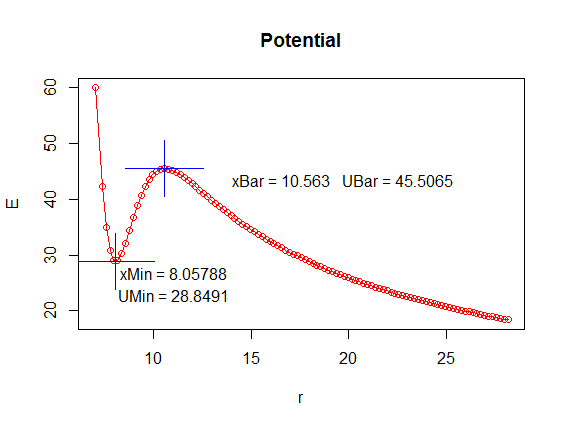
\includegraphics[width=\linewidth]{potential565x427.png}
  \caption{}
  % \caption{A Potential.}
  % \label{fig:Potential}
\end{figure}

\begin{figure}[h!]
  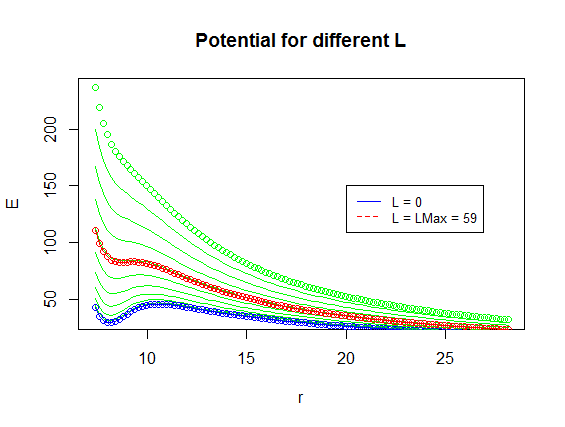
\includegraphics[width=\linewidth]{prob565x427.png}
  \caption{}
  % \caption{A Potential.}
  % \label{fig:Potential for different L}
\end{figure}




  \subsection{Summary for run the program}
  Let us propose all commands step by step for console in Linux system:
        \begin{verbatim}
# path where QDA folder is located:
path='QDA'
# clean files from previous run (if exists): 
rm -f $path/run/*
# compile:
cd $path$/source; 
g++ ./settings.cc -o ../run/settings.exe; \
gfortran P1.FOR P2.FOR P3.FOR P4.FOR \
                 -o ../run/fort.exe; \
g++ pcapt.cc -lgmpxx -lgmp -lmpfr -lgsl -lgslcblas \
             -std=c++11 -o ../run/pcapt.exe ; \
# run:
cd $path/run
./settings.exe  -A1 40 -Z1 20 -A2 40 -Z2 18; 
./fort.exe;
./pcapt.exe; 
# in addition, the following commands run R - scripts for creating graphs:
R CMD BATCH plot.R ;      
R CMD BATCH potential.R;  
R CMD BATCH prob.R ;      
R CMD BATCH ./probd.R ;   
        \end{verbatim}

%% References with bibTeX database:
  % \bibliographystyle{elsarticle-num}
  % \bibliography{<your-bib-database>}
  %% Authors are advised to submit their bibtex database files. They are
  %% requested to list a bibtex style file in the manuscript if they do
  %% not want to use elsarticle-num.bst.


%% References without bibTeX database:
    \end{description} 


\begin{thebibliography}{99}
  \bibitem{poten}     G.G.~Adamian {\it et al.}, Int. J.  Mod. Phys. E {\bf 5}, 191 (1996).
  \bibitem{VVV}       V.V.~Volkov, Phys. Rep. {\bf 44}, 93 (1978).
  \bibitem{Schreder}  W.U.~Schr\"oder and  J.R.~Huizenga, in {\it Treatise~on~Heavy-Ion~Science},
                      Ed. by D.A. Bromley (Plenum, New York, 1984), vol.2, p.115.
  \bibitem{Hofman}    H.~Hofmann, Phys. Rep.  {\bf 284}, 137 (1997);
                      C.~Rummel and H.~Hofmann, Nucl. Phys. A {\bf 727}, 24 (2003).
  %14
  \bibitem{VAZ}       G.G. Adamian, N.V. Antonenko, Z. Kanokov, and V.V. Sargsyan, Teor. Mat. Fiz. {\bf 145}, 87 (2005)
                      [Theor. Math. Phys. {\bf 145}, 1443 (2006)];
                      Z. Kanokov, Yu.V. Palchikov,  G.G. Adamian, N.V. Antonenko, and W. Scheid, Phys. Rev. E {\bf 71}, 016121 (2005);
                      Yu.V. Palchikov, Z. Kanokov,  G.G. Adamian, N.V. Antonenko, and W. Scheid, Phys. Rev. E {\bf 71}, 016122 (2005).
  \bibitem{Ayik}      N.~Takigawa, S.~Ayik, K.~Washiyama, and S.~Kimura, Phys. Rev. C {\bf 69}, 054605 (2004);
                      S.~Ayik, B.~Yilmaz, A. Gokalp, O. Yilmaz, and N.~Takigawa, Phys. Rev. C {\bf 71}, 054611 (2005);
                      B. Yilmaz, S. Ayik, Y. Abe, and D. Boilley, Phys. Rev. E {\bf 77}, 011121 (2008).
  \bibitem{DMDadonov} V.V. Dodonov and V.I. Man'ko, Trudy Fiz. Inst. AN {\bf 167}, 7 (1986);  H.~Dekker, Phys.~Rep. {\bf 80}, 1 (1981);
                      A. Isar, A. Sandulescu, H. Scutaru, E. Stefanescu, and W. Scheid, Int. J. Mod. Phys. E {\bf 3}, 635 (1994);
                      G.G.~Adamian, N.V.~Antonenko, and  W.~Scheid, Phys. Lett. A {\bf 244},  482 (1998);
                      Phys. Lett. A {\bf 260}, 39 (1999); Nucl. Phys. A {\bf 645}, 376 (1999);
                      Yu.V.~Palchikov, G.G.~Adamian, N.V.~Antonenko, and  W.~Scheid, J. Phys. A {\bf 33}, 4265 (2000);
                      Physica A {\bf 316}, 297 (2002).
  \bibitem{Leggett}   A.O. Caldeira, and A.J. Leggett, Physica A. {\bf 121}, 587 (1983); Ann. Phys. {\bf 149} 374 (1983).
  \bibitem{Jolos}     R. V. Jolos, S. P. Ivanova, and V. V. Ivanov, Sov. J. Nucl. Phys. {\bf 40}, 74 (1984);
                      S. P. Ivanova and R. V. Jolos, Nucl. Phys. A. {\bf 530}, 232 (1991).
  \bibitem{Katia}     K. Lindenberg,  and B. West. Phys. Rev. A. {\bf 30}, 568 (1984).
  \bibitem{Kampen}    N.G. van Kampen, {\it Stochastic Processes in Physics and Chemistry}, Amsterdam: North-Holland, 1981.
  \bibitem{Gardiner}  C.W. Gardiner, {\it Quantum Noise}, Berlin: Springer, 1991.
  \bibitem{Weiss}     U. Weiss, {\it Quantum Dissipative Systems}. Singapore: Wold Scientific, 1999.
  \bibitem{Grabert}   H. Grabert, P. Schramm, G.-L. Ingold, Phys. Rep. {\bf 168}, 115 (1988); P. Talkner, Ann. Phys. {\bf 167}, 390 1986.
  \bibitem{PRC1}      G.G. Adamian, A.K. Nasirov, N.V. Antonenko, R.V. Jolos, Phys. Part. Nucl. {\bf 25}, 583 (1994).
  \bibitem{PRC2}      V.V.~Sargsyan, Z.~Kanokov, G.G.~Adamian, N.V.~Antonenko, and W.~Scheid,
                      Phys. Rev. C {\bf 80}, 034606 (2009); Phys. Rev. C {\bf 80}, 047603 (2009).
  \bibitem{Wash}      K. Washiyama, D. Lacroix, S. Ayik, Phys. Rev. C {\bf 79}, 024609 (2009).
  \bibitem{Ayik1}     S. Ayik, K. Washiyama, D. Lacroix, Phys. Rev. C {\bf 79}, 054606 (2009).
  \bibitem{Stelson}   P. H. Stelson, H. J. Kim, M. Beckerman, D. Shapira, and R. L. Robinson, Phys. Rev. C {\bf 41}, 1584 (1990).
  \bibitem{NashiTrs}  V. V. Sargsyan, G. G. Adamian, N. V. Antonenko, W. Scheid, and H. Q. Zhang, Phys. Rev. C {\bf 84}, 064614 (2011);
                      {\bf 85}, 024616 (2012); {\bf 91}, 014613 (2015);
                      V. V. Sargsyan, G. G. Adamian, N. V. Antonenko, W. Scheid, C. J. Lin, and H. Q. Zhang, ibid. 85, 017603 (2012).
  \bibitem{Broglia}   R. A. Broglia, C. H. Dasso, S. Landowne, and A. Winther, Phys. Rev. C 27, 2433 (1983); R. A. Broglia, C. H. Dasso,
                      S. Landowne, and G. Pollarolo, Phys. Lett. B 133, 34 (1983).
  \bibitem{Szilner}   S. Szilner, {\it at al}, Phys. Rev. C {\bf 76}, 024604 (2007); 84, 014325 (2011);
                      L. Corradi, {\it at al}, ibid. {\bf 84}, 034603 (2011).
  \bibitem{Raman}     S. Raman, C.W. Nestor Jr., and P. Tikkanen, At. Data Nucl. Data Tables {\bf 78}, 1 (2001).
  \bibitem{WebInterface}  http://intel-robot.ru/external/www5
  \bibitem{Rscripts}  https://www.r-project.org/

\end{thebibliography}





\end{document}